\section{FIR - Finite Impulse Response}\label{sec:fir}
Formålet med FIR filteret er at udregne filter koefficienterne, $b_{i}$, der bruges til at approksimere størrelsen af frekvens responset af FIR filteret $H(z)$.

\husk{Kenneth}{FIR generelt her}


Forholdet mellem input og output i er FIR filter er givet ved ligning \ref{fir_ligning},
\begin {equation} 
y(n)=\sum\limits_{i=0}^{K}b_{i}x(n-i) \label{fir_ligning}
\end {equation}
hvor $b_{i}$ repræsenterer filterets koefficienter og $K+1$ er filterets længde.
\\
Derefter z-transformeres ligning \ref{fir_ligning}. For at opskrive FIR filterets overføringsfunktion, faktoriseres $X(z)$ ud på højre side af den z-transformerede ligning \ref{fir_ligning} og derefter dividere igennem med $X(z)$ fås ligning \ref{fir_transfer}.

\begin {equation}
H(z)=\frac{Y(z)}{X(z)}=b_{0}+b_{1}z^{-1}+...+b_{K}^{-1} \label{fir_transfer}
\end {equation}

Input og output signalet er givet ved foldning og er opskrevet i ligning,
\begin {equation} 
\sum\limits_{i=0}^{N-1} h(k)x(n-k) 
\end {equation}
hvor $h(k)$ er impulsresponset modsat IIR filterne har en endelig længde, $N$, antal værdier. FIR filterets impulsrespons er et sæt af filter koefficienter. Sendes en impuls ind i filteret bestående af et $"1"$ efterfulgt af mange $"0"$er, bliver filterets output det sæt af koefficienter $"1"$-samplen kører igennem. 


FIR filterets overføringsfunktion er givet ved ligning \ref{FIR_transfer}

\begin {equation}
H(z)=\sum\limits_{k=0}^{N-1}h(k)z^{-1} \label{FIR_transfer}
\end {equation}

\section{Design metoder} \label{sec:fir_design}
\husk{Kenneth}{Mere eller mindre en løsningsmodel, så det kan sammenlignes med IIR implementeringen - teori og praksis}
\husk{Kenneth}{Blokdiagram som løsning}
Herunder redegøres der for 2 forskellíge design metoder, til beregning af filter koefficienter.
Frekvenssamplingsmetoden vil være mere dybdegående end de to andre, da det er den metode der vil blive implementeret.
\subsection{Frekvenssampling}
Ved frekvenssampling approksimeres det ønskede frekvensrespons ved, at sample det $N$ antal gange, med samme interval imellem samplingspunkterne. Der kan derved opnås et interpolateret frekvens respons.
Pointen med frekvenssampling er at filterkoefficienter kan beregnes udfra specificerede størrelser i forhold det ønskede filter respons uniformt i frekvensdomænet.

Filterkoefficienterne kan beregnes udfra definitionen af den inverse DFT (IDFT):

\begin {equation}
h(n)=\frac{1}{N}\sum_{k=0}^{N-1}H_{d}(k)W_{N}^{-kn} ,\hspace{1cm}\text{for}\hspace{1cm} n = 0, 1,\text{ ... }, N-1 \label{fir_filterkoefficienter}
\end {equation}
hvor
\begin {equation}
W_{N}=e^{j\frac{2\pi}{N}} \hspace{1cm}\text{og} \hspace{1cm} H_{d}(k)=h(e^{j\Omega_{k}}) \nonumber
\end {equation}
Det antages lineær fase og at antallet af samplingspunkt er $N=2M+1$.



\begin{figure}[h]
\centering
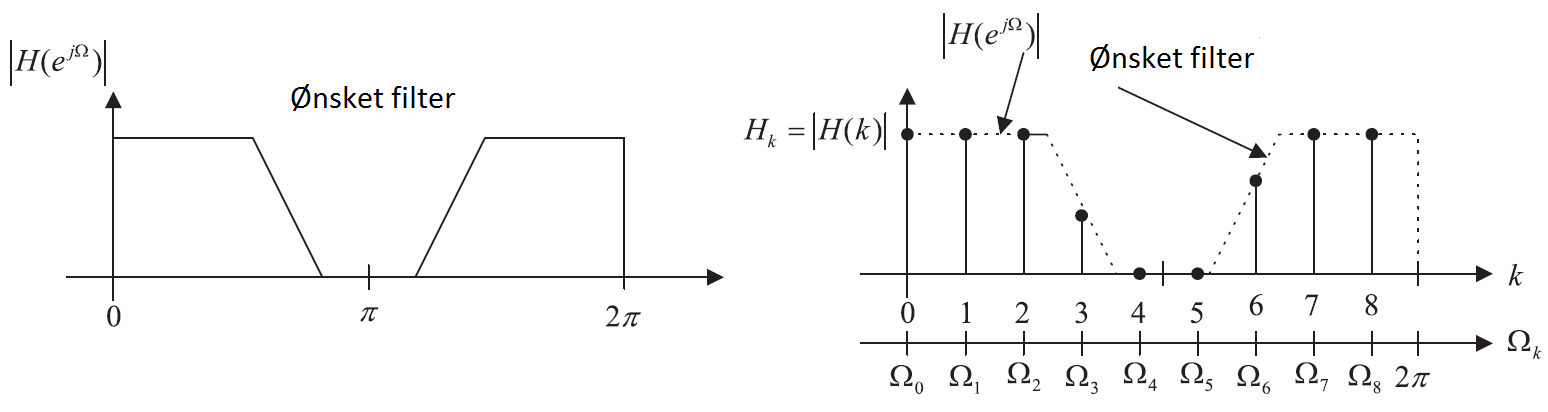
\includegraphics[width=.90\textwidth]{billeder/fir_frekvenssampling.png}\label{fig:fir_frekvenssampling}
\caption{Ønskede filterrespons og samplede filterrespons.}
\end{figure}
\FloatBlock
Ligning \ref{fir_filterkoefficienter} kan simplificeres til,
\begin {equation}
h(n)=\frac{1}{2M+1}\left[ H_{0}+2\sum_{k=1}^{M} \left( \frac{2\pi k(n-M)}{2M+1} \right) \right] \hspace{1cm} \text{for} \hspace{1 cm} n=0,1,\text{ ... },2M
\end {equation}

hvor $h(k)$ for $k=0,1,\text{ ... },2M$, repræsenterer filterkoefficienternes størrelser, der bruges til at specificere det ønskede filterrespons med samplingslængden $\Omega_{k}=\frac{2\pi k}{(2M+1)}$.



\subsection{Windowsmetoden}
\husk{Kenneth}{Blokdiagram - fortælling omkring de forskellige vinduer}
\husk{Kenneth}{Gennemgang af koefficienterne med Fourier}
Den grundlæggende tilgang til windowsmetoden er baseret på at det ideelle lavpas-, højpas-, båndpas-, og båndstop filter, bestående af den følgende ikke-kausale impulsrespons på $-\infty < n < \infty$. Windowsmetoden bygger på Fourier Transformationen, hvor der gælder om at fjerne de uønskede Gibbs oscilleringer i pas- og stopbåndet, som finder sted under trunkeringen. Anvendes windowsmetoden på filterkoefficienterne fås ligning \ref{window_function},
\begin{equation}
	h_w(n) = h(n)*w(n) \hspace{1cm}\text{,} \hspace{1cm}n=-M,\text{ ... },0, 1,\text{ ... , }M	
	\label{window_function}
\end{equation}
hvor $w(n)$ angiver det valgte vindue.

For at beregne koefficienterne for $h_w$ forsinket impuls sekvensen med M samples som ses i ligning \ref{b_n-window}
\begin{equation}
	b_n = h_w (n-M), \hspace{1cm} \text{for} \hspace{1cm} n = 0,1, \text{ ... , }M \label{b_n-window}
\end{equation}

Grundlaget for valg af vindue baseres blandt andet på overgangsbåndet $\Delta f$.

\begin{equation}
\Delta f = \frac{f_{stop}-f_{pas}}{f_s} \label{Windows_transistionband}
\end{equation}

Ripplen er henholdsvis pas- og stopbåndet beregnes udfra ligning \ref{ripple_p} og \ref{ripple_s}.

\begin{align}
\delta_p dB &= 20*log_{10}(1+\delta_p) \label{ripple_p}\\
\delta_s dB &= -20*log_{10}(\delta_s) \label{ripple_s}
\end{align}

Filterets knækfrekvens, $f_c$, bestemmes ud fra midten af overgangsbåndet. En tommmelfingerregel til bestemmelse af $f_c$ er givet ved ligning \ref{fir_cutoff}
\begin{equation}
	f_c =\frac{f_{pas}-f_{stop}}{2} \label{fir_cutoff}
\end{equation}




\begin{equation}
h_{d,LP}[n] = \frac{sin(\omega_c n)}{\pi n} \label{windows_lp}
\end{equation}
\begin{equation}
h_{d,HP}[n] = \delta(n) - \frac{sin(\omega_c n)}{\pi n} \label{windows_hp}
\end{equation}
\begin{equation}
h_{d,BP}[n] = \frac{sin(\omega_b n) - sin(\omega_a n)}{\pi n} \label{windows_bp}
\end{equation}
\begin{equation}
h_{d,BS}[n] = \delta(n) - \frac{sin(\omega_b n) - sin(\omega_a n)}{\pi n} \label{windows_bs}
\end{equation}

Ligningerne \ref{windows_lp}, \ref{windows_hp}, \ref{windows_bp} og \ref{windows_bs} er de generelle filterfunktioner. Efter valget af hvilken filtertype der skal anvendes, findes det nødvendige vindue, at påtrykke filteret med.


\section{Opsummering}

\husk{Kenneth}{Sammenligning af de to metoder, samt nævne at der findes flere metoder.}
